\begin{figure}[t]
\centering
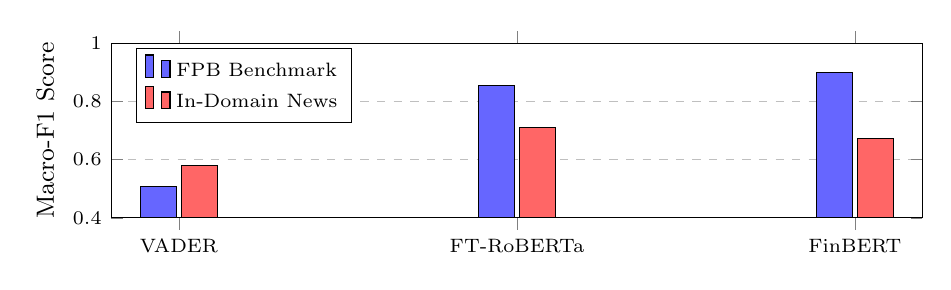
\begin{tikzpicture}
\begin{axis}[
    ybar,
    width=0.98\columnwidth,
    height=3.8cm,
    bar width=13pt,
    ylabel={Macro-F1 Score},
    symbolic x coords={VADER, FT-RoBERTa, FinBERT},
    xtick=data,
    ymin=0.4, ymax=1.0,
    legend pos=north west,
    legend style={font=\scriptsize},
    label style={font=\small},
    tick label style={font=\scriptsize},
    ymajorgrids=true,
    grid style=dashed
]
\addplot[fill=blue!60] coordinates {(VADER, 0.507) (FT-RoBERTa, 0.854) (FinBERT, 0.898)};
\addlegendentry{FPB Benchmark}
\addplot[fill=red!60] coordinates {(VADER, 0.581) (FT-RoBERTa, 0.711) (FinBERT, 0.672)};
\addlegendentry{In-Domain News}
\end{axis}
\end{tikzpicture}
\caption{Cross-Domain Generalization Gap across Sentiment Models. Transferring models to general journalistic headlines induces a 16.8\% relative drop for DistilRoBERTa and a 25.2\% drop for FinBERT.}
\label{fig:domain_gap}
\end{figure}